
\section{Introduction}

DNA usually evolves by tiny mutations. However, sometimes something more radical happens, and the order of a contiguous segment of genome is rearranged. Understanding these rearrangement sheds light on the process of evolution. Every genome rearrangement results in a change of gene ordering, and a
series of these rearrangements can alter the genomic architecture of a species. Biologists are interested in the most parsimonious evolutionary scenario,
that is, the scenario involving the smallest number of reversals. While there is
no guarantee that this scenario represents an actual evolutionary sequence, it
gives us a lower bound on the number of rearrangements that have occurred
and indicates the similarity between two species.
\subsection{Human and Mice}

In some ways, the
human genome is just the mouse genome cut into about 300 large genomic
fragments, called synteny blocks, that have been pasted together in a different
order. Both sequences are just two different shufflings of the ancient mammalian genome. 

\begin{figure}[h] 
	\center 
	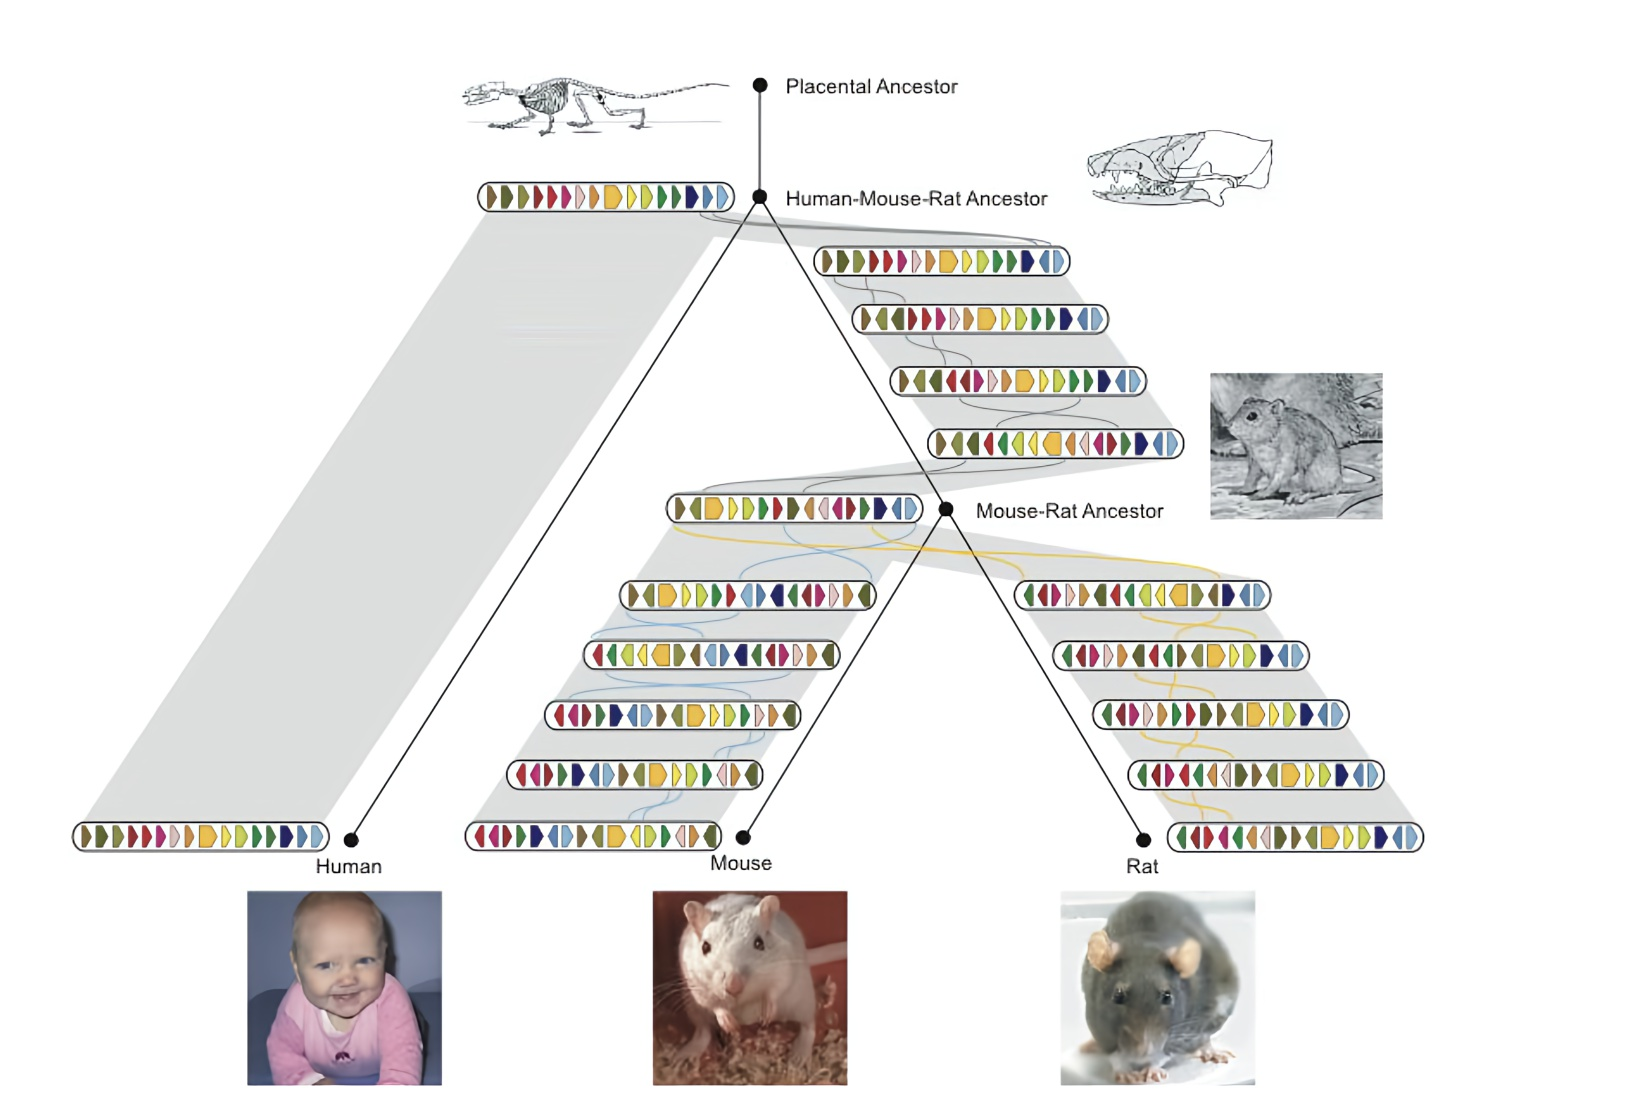
\includegraphics[width=0.7\linewidth]{assets/evolutionary_tree.jpg}
    \captionsetup{justification=centering, font=small}
	\caption{Evolutionary tree of mouse, rat, and human showing genome rearrangements\protect\footnotemark{}} 
\end{figure}

\begin{figure}[h] 
	\center 
	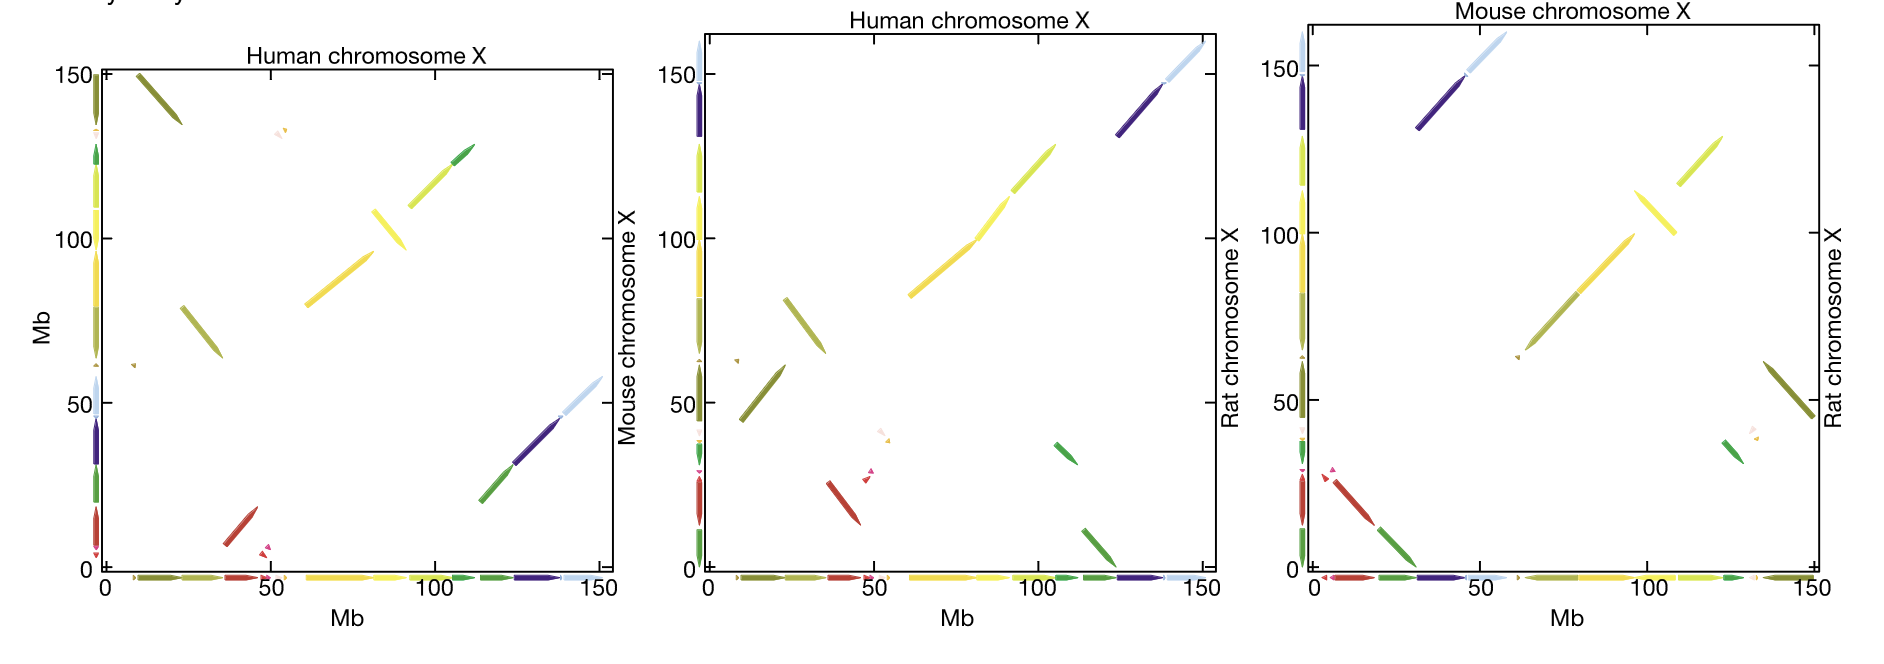
\includegraphics[width=0.7\linewidth]{assets/sentry_block.png}
    \captionsetup{justification=centering, font=small}
	\caption{sentry block alignments of each pair of species } 
\end{figure}



\footnotetext{Extreme conservation of genes on X chromosomes across mammalian species provides an
opportunity to study the evolutionary history of X chromosomes independently of the rest of the
genomes, since the gene content of X chromosomes has barely changed throughout mammalian
evolution. However, the order of genes on X chromosomes has been disrupted several times. In
other words, genes that reside on the X chromosome stay on the X chromosome (but their order
may change). All other chromosomes may exchange genes, that is, a gene can move from one
chromosome to another.} 



\subsection{Combinatorial Problems}

Every study of genome rearrangements involves solving the combinatorial puzzle of finding a series of rearrangements that transform one genome into another. Due to the parsimonious nature of evolution, we are interested in the minimum number of steps in which one genome sequence can be transformed into the other using only reversals, the most common evolutionary event. 
\subsubsection{Sorting by Reversals}
In the simplest form, the order of genes can be represented by a permutation  $ \pi = \pi_{1} \pi_{2} \ldots \pi_{n} $. We define a reversal $ \rho (i, j) $ transforms permutation in the following way 
\begin{center}
$ \pi = \pi_{1} \pi_{2} \ldots \pi_{i} \pi_{i+1} \ldots \pi_{j} \pi_{j+1}  \ldots \pi_{n} $ \\ 
$ \pi . \rho (i, j) = \pi_{1} \pi_{2} \ldots \pi_{j} \pi_{j-1} \ldots \pi_{i-1} \pi_{i} \ldots \pi_{n} $.
\end{center}

In the sorting by reversals problem, we are interested in applying a number of reversals $ \rho_1 \rho_2 \ldots \rho_n $ to transform permutation $ \pi $ into the identity permutation.

\subsubsection{Pancake Problem}

In 1975, Jacob E. Goodman (under the pseudonym Harry Dweighter) posed the following problem:
\begin{quote}
The chef in our place is sloppy, and when he prepares a stack of pancakes they come out all different sizes. Therefore, when I deliver them to a customer, on the way to the table I rearrange them (so that the smallest winds up on top, and so on, down to the largest at the bottom) by grabbing several from the top and flipping them over, repeating this (varying the number I flip) as many times as necessary. If there are n pancakes, what is the maximum number of flips (in terms of n) that I will ever have to use to rearrange them?
\end{quote}
The Pancake Problem, is also know as Sorting by Prefix Reversals. In this setting we can only apply reversals that start from the beginning of the sequence, $ \rho (1, j) $ or simply $\rho(j)$ in this case. 

\subsubsection{Bounds for Pancake Flipping Problem}
On obvious algorithm for sorting the permutation is as follows:  Given permutation $ \pi $ assume that the elements $ \pi_i \pi_{i+1} \ldots \pi_{n} $ are already in the correct order for $ 1 \leq i \leq n $. If $ i = 1 $ the permutation is already sorted, hence we assume that $ i > 1$. We denote the position of $ i-1 $ by  $ \pi_{j} $, and perform the reversal operations $ \rho(\pi_{j}).\rho(\pi_{i-1})$. 
Thus, we can put each element in its correct position by 2 operations. Since we only need to put $n - 1$ elements in their correct position, this algorithms sorts any permutation in at most $2(n-1)$ operations. In 1979, Gates and Papadimitriou \cite{bounds} improved bounds for the pancake flipping problem. In this report, we'll examine their presented algorithm, that sorts any permutation in at most $\frac{5}{3}(n+1)$ steps. 

\subsubsection{Related Work}
The MIN-SBR problem has been shown to be NP-Complete by Caprara \cite{caprara}. However, Hannenhalli and Pevzner \cite{cabbages_into_turnips} gave an exact polynomial time algorithm for a slightly restricted version of the problem. In 2011, Laurent Bulteau, Guillaume Fertin, and Irena Rusu \cite{pancake-flipping-is-hard} showed that MIN-SBPR is also NP-Complete, thereby answering a question that had been open for over three decades.
